\begin{frame}{Transferencias del GNC para pensiones y asignaciones de retiro}
\begin{center}
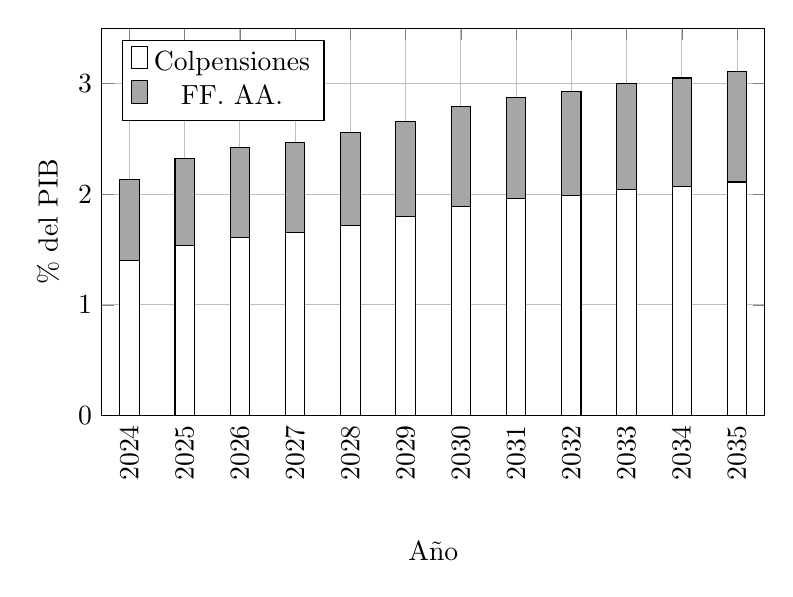
\begin{tikzpicture}
    \begin{axis}[
        width=10cm, height=6.5cm,
        xlabel={Año},
        ylabel={\% del PIB},
        xtick=data,
        ymin=0, ymax=3.5,
        legend pos=north west,
        grid=major,
        xticklabels={2024, 2025, 2026, 2027, 2028, 2029, 2030, 2031, 2032, 2033, 2034, 2035},
        xticklabel style={rotate=90, anchor=east},
        xlabel style={yshift=-15pt},
        ybar stacked,
        bar width=7pt,
        enlarge x limits={abs=0.5},
        nodes near coords style={font=\small}
    ]
    
    % Colpensiones
    \addplot[fill=white, draw=black] coordinates {
        (2024,1.40) (2025,1.54) (2026,1.61) 
        (2027,1.65) (2028,1.72) (2029,1.80) (2030,1.89) (2031,1.96) 
        (2032,1.99) (2033,2.04) (2034,2.07) (2035,2.11)
    };
    \addlegendentry{Colpensiones}
    
    % FF.AA.
    \addplot[fill=gray!70] coordinates {
        (2024,0.73) (2025,0.78) (2026,0.81) 
        (2027,0.82) (2028,0.84) (2029,0.86) (2030,0.90) (2031,0.91) 
        (2032,0.94) (2033,0.96) (2034,0.98) (2035,1.00)
    };
    \addlegendentry{FF. AA.}
    
    \end{axis}
\end{tikzpicture}
\end{center}
%\vspace{0.2cm}
%{\footnotesize\textit{Fuente: Marco Fiscal de Mediano Plazo 2024, Ministerio de Hacienda.}}
\end{frame}
